%-----------------------------------
% Define document and include general packages
%-----------------------------------
% Tabellen- und Abbildungsverzeichnis stehen normalerweise nicht im
% Inhaltsverzeichnis. Gleiches gilt für das Abkürzungsverzeichnis (siehe unten).
% Manche Dozenten bemängeln das. Die Optionen 'listof=totoc,bibliography=totoc'
% geben das Tabellen- und Abbildungsverzeichnis im Inhaltsverzeichnis (toc=Table
% of Content) aus.
% Da es aber verschiedene Regelungen je nach Dozent geben kann, werden hier
% beide Varianten dargestellt.
\documentclass[12pt,oneside,titlepage,listof=totoc,bibliography=totoc]{scrartcl}
%\documentclass[12pt,oneside,titlepage]{scrartcl}

%-----------------------------------
% Dokumentensprache
%-----------------------------------
%\def\FOMEN{}% Auskommentieren um die Dokumentensprache auf englisch zu ändern
\newif\ifde
\newif\ifen

%-----------------------------------
% Meta informationen
%-----------------------------------
%-----------------------------------
% Meta Informationen zur Arbeit
%-----------------------------------

% Autor
\newcommand{\myAutor}{Luis Pflamminger}

% Titel der Arbeit
\newcommand{\myTitel}{Prinzipien und Chancen des DevOps-Konzepts}

% Betreuer
\newcommand{\myBetreuer}{Stiven Raso}

% Lehrveranstaltung
\newcommand{\myLehrveranstaltung}{Software Engineering}

% Matrikelnummer
\newcommand{\myMatrikelNr}{538276}

% Ort
\newcommand{\myOrt}{Düsseldorf}

% Datum der Abgabe
\newcommand{\myAbgabeDatum}{24. Februar 2022}

% Semesterzahl
\newcommand{\mySemesterZahl}{5}

% Name der Hochschule
\newcommand{\myHochschulName}{FOM Hochschule für Oekonomie \& Management}

% Standort der Hochschule
\newcommand{\myHochschulStandort}{Düsseldorf}

% Studiengang
\newcommand{\myStudiengang}{"Wirtschaftsinformatik"}

% Art der Arbeit
\newcommand{\myThesisArt}{Scientific Essay}

% Zu erlangender akademische Grad
\newcommand{\myAkademischerGrad}{Bachelor of Science (B.Sc.)}

% Firma
\newcommand{\myFirma}{Deutsche Telekom AG}


\ifdefined\FOMEN
%Englisch
\entrue
\usepackage[english]{babel}
\else
%Deutsch
\detrue
\usepackage[ngerman]{babel}
\fi


\newcommand{\langde}[1]{%
   \ifde\selectlanguage{ngerman}#1\fi}
\newcommand{\langen}[1]{%
   \ifen\selectlanguage{english}#1\fi}
\usepackage[utf8]{luainputenc}
\langde{\usepackage[babel,german=quotes]{csquotes}}
\langen{\usepackage[babel,english=british]{csquotes}}
\usepackage[T1]{fontenc}
\usepackage{fancyhdr}
\usepackage{fancybox}
\usepackage[a4paper, left=4cm, right=2cm, top=4cm, bottom=2cm]{geometry}
\usepackage{graphicx}
\usepackage{subfig}
\usepackage{wrapfig}
\usepackage{colortbl}
\usepackage[capposition=top]{floatrow}
\usepackage{array}
\usepackage{float}      %Positionierung von Abb. und Tabellen mit [H] erzwingen
\usepackage{footnote}
% Darstellung der Beschriftung von Tabellen und Abbildungen (Leitfaden S. 44)
% singlelinecheck=false: macht die Caption linksbündig (statt zentriert)
% labelfont auf fett: (Tabelle x.y:, Abbildung: x.y)
% font auf fett: eigentliche Bezeichnung der Abbildung oder Tabelle
% Fettschrift laut Leitfaden 2018 S. 45
\usepackage[singlelinecheck=false, labelfont=bf, font=bf]{caption}
\usepackage{caption}
\usepackage{enumitem}
\usepackage{amssymb}
\usepackage{mathptmx}
%\usepackage{minted} %Kann für schöneres Syntax Highlighting genutzt werden. ACHTUNG: Python muss installiert sein.
\usepackage[scaled=0.9]{helvet} % Behebt, zusammen mit Package courier, pixelige Überschriften. Ist, zusammen mit mathptx, dem times-Package vorzuziehen. Details: https://latex-kurs.de/fragen/schriftarten/Times_New_Roman.html
\usepackage{courier}
\usepackage{amsmath}
\usepackage[table]{xcolor}
\usepackage{marvosym}			% Verwendung von Symbolen, z.B. perfektes Eurozeichen

\renewcommand\familydefault{\sfdefault}
\usepackage{ragged2e}

% Mehrere Fussnoten nacheinander mit Komma separiert
\usepackage[hang,multiple]{footmisc}
\setlength{\footnotemargin}{1em}

% todo Aufgaben als Kommentare verfassen für verschiedene Editoren
\usepackage{todonotes}

% Verhindert, dass nur eine Zeile auf der nächsten Seite steht
\setlength{\marginparwidth}{2cm}
\usepackage[all]{nowidow}

%-----------------------------------
% Farbdefinitionen
%-----------------------------------
\definecolor{darkblack}{rgb}{0,0,0}
\definecolor{dunkelgrau}{rgb}{0.8,0.8,0.8}
\definecolor{hellgrau}{rgb}{0.0,0.7,0.99}
\definecolor{mauve}{rgb}{0.58,0,0.82}
\definecolor{dkgreen}{rgb}{0,0.6,0}

%-----------------------------------
% Pakete für Tabellen
%-----------------------------------
\usepackage{epstopdf}
\usepackage{nicefrac} % Brüche
\usepackage{multirow}
\usepackage{rotating} % vertikal schreiben
\usepackage{mdwlist}
\usepackage{tabularx}% für Breitenangabe#
\usepackage{booktabs}

%-----------------------------------
% sauber formatierter Quelltext
%-----------------------------------
\usepackage{listings}
% JavaScript als Sprache definieren:
\lstdefinelanguage{JavaScript}{
	keywords={break, super, case, extends, switch, catch, finally, for, const, function, try, continue, if, typeof, debugger, var, default, in, void, delete, instanceof, while, do, new, with, else, return, yield, enum, let, await},
	keywordstyle=\color{blue}\bfseries,
	ndkeywords={class, export, boolean, throw, implements, import, this, interface, package, private, protected, public, static},
	ndkeywordstyle=\color{darkgray}\bfseries,
	identifierstyle=\color{black},
	sensitive=false,
	comment=[l]{//},
	morecomment=[s]{/*}{*/},
	commentstyle=\color{purple}\ttfamily,
	stringstyle=\color{red}\ttfamily,
	morestring=[b]',
	morestring=[b]"
}

\lstset{
	%language=JavaScript,
	numbers=left,
	numberstyle=\tiny,
	numbersep=5pt,
	breaklines=true,
	showstringspaces=false,
	frame=single ,
	xleftmargin=5pt,
	xrightmargin=5pt,
	basicstyle=\ttfamily\scriptsize,
	stepnumber=1,
	keywordstyle=\color{blue},          % keyword style
  	commentstyle=\color{dkgreen},       % comment style
  	stringstyle=\color{mauve}         % string literal style
}

%-----------------------------------
%Literaturverzeichnis Einstellungen
%-----------------------------------

% Biblatex

\usepackage{url}
\urlstyle{same}

%%%% Neuer Leitfaden (2018)
\usepackage[
backend=biber,
style=ieee,
maxcitenames=3,	% mindestens 3 Namen ausgeben bevor et. al. kommt
maxbibnames=999,
date=iso,
seconds=true, %werden nicht verwendet, so werden aber Warnungen unterdrückt.
urldate=iso,
dashed=false,
autocite=inline,
useprefix=true, % 'von' im Namen beachten (beim Anzeigen)
mincrossrefs = 1
]{biblatex}%iso dateformat für YYYY-MM-DD

%weitere Anpassungen für BibLaTex
%\usepackage{xpatch}

\setlength\bibhang{1cm}

%%% Weitere Optionen
%\boolitem[false]{citexref} %Wenn incollection, inbook, inproceedings genutzt wird nicht den zugehörigen parent auch in Literaturverzeichnis aufnehmen

%Aufräumen die Felder werden laut Leitfaden nicht benötigt.
\AtEveryBibitem{%
\ifentrytype{book}{
    \clearfield{issn}%
    \clearfield{doi}%
    \clearfield{isbn}%
    \clearfield{url}
    \clearfield{eprint}
}{}
\ifentrytype{collection}{
  \clearfield{issn}%
  \clearfield{doi}%
  \clearfield{isbn}%
  \clearfield{url}
  \clearfield{eprint}
}{}
\ifentrytype{incollection}{
  \clearfield{issn}%
  \clearfield{doi}%
  \clearfield{isbn}%
  \clearfield{url}
  \clearfield{eprint}
}{}
\ifentrytype{article}{
  \clearfield{issn}%
  \clearfield{doi}%
  \clearfield{isbn}%
  \clearfield{url}
  \clearfield{eprint}
}{}
\ifentrytype{inproceedings}{
  \clearfield{issn}%
  \clearfield{doi}%
  \clearfield{isbn}%
  \clearfield{url}
  \clearfield{eprint}
}{}
}

\renewcommand*{\finentrypunct}{}%Kein Punkt am ende des Literaturverzeichnisses

\renewcommand*{\newunitpunct}{\addcomma\space}
\DeclareDelimFormat[bib,biblist]{nametitledelim}{\addcolon\space}
\DeclareDelimFormat{titleyeardelim}{\newunitpunct}
%Namen kursiv schreiben
\renewcommand*{\mkbibnamefamily}{\mkbibemph}
\renewcommand*{\mkbibnamegiven}{\mkbibemph}
\renewcommand*{\mkbibnamesuffix}{\mkbibemph}
\renewcommand*{\mkbibnameprefix}{\mkbibemph}

% Die Trennung mehrerer Autorennamen erfolgt durch Kommata.
% siehe Beispiele im Leitfaden S. 16
% Die folgende Zeile würde mit Semikolon trennen
%\DeclareDelimFormat{multinamedelim}{\addsemicolon\addspace}

%Delimiter für mehrere und letzten Namen gleich setzen
\DeclareDelimAlias{finalnamedelim}{multinamedelim}

\DeclareNameAlias{default}{family-given}
\DeclareNameAlias{sortname}{default}  %Nach Namen sortieren


\DeclareFieldFormat{editortype}{\mkbibparens{#1}}
\DeclareDelimFormat{editortypedelim}{\addspace}
\DeclareFieldFormat{translatortype}{\mkbibparens{#1}}
\DeclareDelimFormat{translatortypedelim}{\addspace}
\DeclareDelimFormat[bib,biblist]{innametitledelim}{\addcomma\space}

\DeclareFieldFormat*{citetitle}{#1}
\DeclareFieldFormat*{title}{#1}
\DeclareFieldFormat*{booktitle}{#1}
\DeclareFieldFormat*{journaltitle}{#1}

\xpatchbibdriver{online}
  {\usebibmacro{organization+location+date}\newunit\newblock}
  {}
  {}{}

\DeclareFieldFormat[online]{date}{\mkbibparens{#1}}
\DeclareFieldFormat{urltime}{\addspace #1\addspace \langde{Uhr}\langen{MEZ}}
\DeclareFieldFormat{urldate}{%urltime zu urldate hinzufügen
  [\langde{Zugriff}\langen{Access}\addcolon\addspace
  #1\printfield{urltime}]
}
\DeclareFieldFormat[online]{url}{<\url{#1}>}
\renewbibmacro*{url+urldate}{%
  \usebibmacro{url}%
  \ifentrytype{online}
    {\setunit*{\addspace}%
     \iffieldundef{year}
       {\printtext[date]{\langde{keine Datumsangabe}\langen{no Date} }}
       {\usebibmacro{date}}}%
    {}%
  \setunit*{\addspace}%
  \usebibmacro{urldate}
  }

%Verhindern, dass bei mehreren Quellen des gleichen Autors im gleichen Jahr
%Buchstaben nach der Jahreszahl angezeigt werden wenn sich das Keyword in usera unterscheidet.
\DeclareExtradate{
  \scope{
    \field{labelyear}
    \field{year}
    }
    \scope{
      \field{usera}
     }
}

%% Anzeige des Jahres nach dem Stichwort (usera) im Literaturverzeichnis
%% Wenn das Jahr bei Online-Quellen nicht explizit angegeben wurde, wird nach
%% dem Stichwort 'o. J.' ausgegeben. Nach der URL steht dann 'keine
%% Datumsangabe'. Ist das Jahr definiert, wird es an beiden Stellen ausgegeben.
%% Das Zugriffsdatum (urldate) spielt hier keine Rolle.
%% Für Nicht-Online-Quellen wird nichts geändert.
\renewbibmacro*{date+extradate}{%
  \printtext[parens]{%
    \printfield{usera}%
    \setunit{\printdelim{titleyeardelim}}%
    \ifentrytype{online}
       {\setunit*{\addspace\addcomma\addspace}%
         \iffieldundef{year}
           {\bibstring{nodate}}
       {\printlabeldateextra}}%
       {\printlabeldateextra}}}

%% Anzeige des Jahres nach dem Stichwort (usera) in der Fussnote
%% das Stichwort hat der Aufrufer hier schon ausgegeben.
%% siehe auch Kommentar zu: \renewbibmacro*{date+extradate}
\renewbibmacro*{cite:labeldate+extradate}{%
    \ifentrytype{online}
       {\setunit*{\addspace\addcomma\addspace}%
         \iffieldundef{year}
           {\bibstring{nodate}}
       {\printlabeldateextra}}%
       {\printlabeldateextra}}


\DefineBibliographyStrings{german}{
  nodate    = {{}o.\adddot\addspace J\adddot},
  andothers = {et\addabbrvspace al\adddot}
}
\DefineBibliographyStrings{english}{
  nodate    = {{}n.\adddot\addspace d\adddot},
  andothers = {et\addabbrvspace al\adddot}
}
\DeclareSourcemap{
  \maps[datatype=bibtex]{
    \map{
      \step[notfield=translator, final]
      \step[notfield=editor, final]
      \step[fieldset=author, fieldvalue={{{\langde{o\noexpand\adddot\addspace V\noexpand\adddot}\langen{Anon}}}}]
    }
    \map{
      \pernottype{online}
      \step[fieldset=location, fieldvalue={\langde{o\noexpand\adddot\addspace O\noexpand\adddot}\langen{s\noexpand\adddot I\noexpand\adddot}}]
    }
  }
}

\renewbibmacro*{cite}{%
  \iffieldundef{shorthand}
    {\ifthenelse{\ifnameundef{labelname}\OR\iffieldundef{labelyear}}
       {\usebibmacro{cite:label}%
        \setunit{\printdelim{nonametitledelim}}}
       {\printnames{labelname}%
        \setunit{\printdelim{nametitledelim}}}%
     \printfield{usera}%
     \setunit{\printdelim{titleyeardelim}}%
     \usebibmacro{cite:labeldate+extradate}}
    {\usebibmacro{cite:shorthand}}}

    \renewcommand*{\jourvoldelim}{\addcomma\addspace}% Trennung zwischen journalname und Volume. Sonst Space; Laut Leitfaden richtig
    %Aufgrund der Änderung bzgl des Issues 169 in der thesis_main.tex musste ich die Zeile auskommentieren. Konnte aber das Verhalten, dass die Fußnoten grün sind, im nachhinein nicht feststellen.
    %\hypersetup{hidelinks} %sonst sind Fußnoten grün. Dadurch werden Links allerdings nicht mehr farbig dargestellt

\renewbibmacro*{journal+issuetitle}{%
  \usebibmacro{journal}%
  \setunit*{\jourvoldelim}%
  \iffieldundef{series}
    {}
    {\setunit*{\jourserdelim}%
     \printfield{series}%
     \setunit{\servoldelim}}%
  \iffieldundef{volume}
    {}
    {\printfield{volume}}
  \iffieldundef{labelyear}
  {}
  {
  (\thefield{year}) %Ansonsten wird wenn kein Volume angegeben ist ein Komma vorangestellt
  }
  \setunit*{\addcomma\addspace Nr\adddot\addspace}
  \printfield{number}
  \iffieldundef{eid}
  {}
  {\printfield{eid}}
}

% Postnote ist der Text in der zweiten eckigen Klammer bei einem Zitat
% wenn es keinen solchen Eintrag gibt, dann auch nicht ausgeben, z.B. 'o. S.'
% Wenn man das will, kann man das 'o. S.' ja explizit angeben. Andernfalls steht
% sonst auch bei Webseiten 'o. S.' da, was laut Leitfaden nicht ok ist.
\renewbibmacro*{postnote}{%
  \setunit{\postnotedelim}%
  \iffieldundef{postnote}
    {} %{\printtext{\langde{o.S\adddot}\langen{no page number}}}
    {\printfield{postnote}}}

% Abstand bei Änderung Anfangsbuchstabe ca. 1.5 Zeilen
\setlength{\bibinitsep}{0.75cm}

% nur in den Zitaten/Fussnoten den Vornamen abkürzen (nicht im
% Literaturverzeichnis)

\DeclareDelimFormat{nonameyeardelim}{\addcomma\space}
\DeclareDelimFormat{nameyeardelim}{\addcomma\space}

\renewbibmacro*{cite}{%
  \iffieldundef{shorthand}
    {\ifthenelse{\ifciteibid\AND\NOT\iffirstonpage}
       {\usebibmacro{cite:ibid}}
    {\printtext[bibhyperref]{\ifthenelse{\ifnameundef{labelname}\OR\iffieldundef{labelyear}}
       {\usebibmacro{cite:label}%
        \setunit{\printdelim{nonameyeardelim}}}
      {\toggletrue{abx@bool@giveninits}%
        \printnames[family-given]{labelname}%
        \setunit{\printdelim{nameyeardelim}}}%
      \printfield{usera}%
      \setunit{\printdelim{titleyeardelim}}%
     \usebibmacro{cite:labeldate+extradate}}}}
   {\usebibmacro{cite:shorthand}}}

%% et al. anstatt u. a. bei mehr als drei Autoren.
\DefineBibliographyStrings{ngerman}{ 
	andothers = {{et\,al\adddot}},             
}
\DefineBibliographyStrings{english}{ 
	andothers = {{et\,al\adddot}},             
}


%%%%% Alter Leitfaden. Ggf. Einkommentieren und Bereich hierüber auskommentieren
%\usepackage[
%backend=biber,
%style=numeric,
%citestyle=authoryear,
%url=false,
%isbn=false,
%notetype=footonly,
%hyperref=false,
%sortlocale=de]{biblatex}

%weitere Anpassungen für BibLaTex
%% Optionen für Biblatex
\ExecuteBibliographyOptions{%
giveninits=false,
isbn=true,
url=true,
doi=false,
eprint=false,
maxbibnames=7, % Alle Autoren (kein et al.)
maxcitenames=2, % et al. ab dem 3. Autor
backref=false, % Rückverweise auf Zitatseiten
bibencoding=utf8, % wenn .bib in utf8, sonst ascii
bibwarn=true, % Warnung bei fehlerhafter bib-Datei
}%

% et al. an Stelle von u.a.
\DefineBibliographyStrings{ngerman}{
   andothers = {{et\,al\adddot}},
}

% Klammern um das Jahr in der Fußnote
\renewbibmacro*{cite:labelyear+extrayear}{%
  \iffieldundef{labelyear}
    {}
    {\printtext[bibhyperref]{%
       \mkbibparens{%
         \printfield{labelyear}%
         \printfield{extrayear}}}}}

\renewbibmacro*{cite:title}{%
  \printtext[bibhyperref]{%
    \printfield[citetitle]{labeltitle}%
    \setunit{\addcomma\space}%
    \printdate}}

\DeclareNameFormat{last-first}{%
  \iffirstinits
    {\usebibmacro{name:family-given}
        {\namepartfamily}
        {\namepartgiveni}
        {\namepartprefix}
        {\namepartsuffix}
    }
    {\usebibmacro{name:family-given}
        {\namepartfamily}
        {\namepartgiven}
        {\namepartprefix}
        {\namepartsuffix}
    }%
  \usebibmacro{name:andothers}}

% Alternative Notation der Fußnoten
% Zeigt sowohl den Nachnamen als auch den Vornamen an
% Beispiel: \fullfootcite[Vgl. ][Seite 5]{Tanenbaum.2003}
\DeclareCiteCommand{\fullfootcite}[\mkbibfootnote]
  {\usebibmacro{prenote}}
  {\usebibmacro{citeindex}%
    \printnames[sortname][1-1]{author}%
    \addspace (\printfield{year})}
  {\addsemicolon\space}
  {\usebibmacro{postnote}}

%Autoren (Nachname, Vorname)
\DeclareNameAlias{default}{family-given}

%Reihenfolge von publisher, year, address verändern
% Achtung, bisher nur für den Typ @book definiert

%% Definiert @Book Eintrag
\DeclareBibliographyDriver{book}{%
  \printnames{author}%
  \newunit\addcolon\space
  \printfield{title}%
  \setunit*{,\space}%
  \printfield{edition}%
  \setunit*{\addcomma\space}%
  \printlist{publisher}%
  \newunit\newblockpunct
  \printlist{location}%
  \setunit*{\space}%
  \printfield{year}%
  \setunit*{,\space}%
  \printfield{isbn}%
  \finentry}

%% Definiert @Online Eintrag
\DeclareBibliographyDriver{online}{%
  \printnames{author}%
  \newunit\newblockpunct
  \printfield{title}%
  \setunit*{,\space}%
  %\newunit\newblock
  \printfield{url}%
  \setunit*{,\space Erscheinungsjahr:\space}%
  \printfield{year}%
  \setunit*{,\space Aufruf am:\space}%
  \printfield{note}%
  \finentry}

%% Definiert @Article Eintrag
\DeclareBibliographyDriver{article}{%
  \printnames{author}%
  \newunit\newblockpunct
  \printfield{title}%
  \setunit*{.\space In:\space}%
  %\newunit\newblock
  \usebibmacro{journal}%
  \setunit*{\space (}%
  \printfield{year}\newunit{)}%
  \finentry}

%% Definiert @InProceedings Eintrag
\DeclareBibliographyDriver{inproceedings}{%
	\printnames{author}%
	\setunit*{,\space (}%
	\printfield{year}\newunit{)}%
	\newunit\newblockpunct
	\printfield{title}%
	\setunit*{\space}%
	\usebibmacro{booktitle}%
	\setunit*{,\space}%
	\printfield{isbn}%
	\setunit*{,\space}%
	\printfield{doi}%
	\finentry}

%Doppelpunkt nach dem letzten Autor
\renewcommand*{\labelnamepunct}{\addcolon\addspace }

%Komma an Stelle des Punktes
\renewcommand*{\newunitpunct}{\addcomma\space}

%Autoren durch Semikolon trennen
\newcommand*{\bibmultinamedelim}{\addsemicolon\space}%
\newcommand*{\bibfinalnamedelim}{\addsemicolon\space}%
\AtBeginBibliography{%
  \let\multinamedelim\bibmultinamedelim
  \let\finalnamedelim\bibfinalnamedelim
}

%Titel nicht kursiv anzeigen
\DeclareFieldFormat{title}{#1\isdot}


%%%% Ende Alter Leitfaden

%Bib-Datei einbinden
\addbibresource{literature/literature.bib}

% Zeilenabstand im Literaturverzeichnis ist Einzeilig
% siehe Leitfaden S. 14
\AtBeginBibliography{\singlespacing}

%-----------------------------------
% Silbentrennung
%-----------------------------------
\usepackage{hyphsubst}
\HyphSubstIfExists{ngerman-x-latest}{%
\HyphSubstLet{ngerman}{ngerman-x-latest}}{}

%-----------------------------------
% Pfad fuer Abbildungen
%-----------------------------------
\graphicspath{{./}{./figures/}}

%-----------------------------------
% Weitere Ebene einfügen
%-----------------------------------
\usepackage{titletoc}

\makeatletter

% Setze die Tiefe des Inhaltsverzeichnis auf 4 Ebenen
% Damit erscheinen \paragraph-Sektionen auch im Inhaltsverzeichnis
\setcounter{secnumdepth}{4}
\setcounter{tocdepth}{4}

% Fuege Abstand nach unten wie in einer normalen \section hinzu
% Andernfalls haette \paragraph keinen Zeilenumbruch
% Der Zeilenumbruch koennte mit einer leeren \mbox{} ersetzt werden
% Jedoch klebt dann der Text relativ nah an der Ueberschrift
\renewcommand{\paragraph}{%
  \@startsection{paragraph}{4}%
  {\z@}{3.25ex \@plus 1ex \@minus .2ex}{1.5ex plus 0.2ex}%
  {\normalfont\normalsize\bfseries\sffamily}%
}

\makeatother


%-----------------------------------
% Paket für die Nutzung von Anhängen
%-----------------------------------
\usepackage{appendix}

%-----------------------------------
% Zeilenabstand 1,5-zeilig
%-----------------------------------
\usepackage{setspace}
\onehalfspacing

%-----------------------------------
% Absätze durch eine neue Zeile
%-----------------------------------
\setlength{\parindent}{0mm}
\setlength{\parskip}{0.8em plus 0.5em minus 0.3em}

\sloppy					%Abstände variieren
\pagestyle{headings}

%----------------------------------
% Präfix in das Abbildungs- und Tabellenverzeichnis aufnehmen, statt nur der Nummerierung (siehe Issue #206).
%----------------------------------
\KOMAoption{listof}{entryprefix} % Siehe KOMA-Script Doku v3.28 S.153
\BeforeStartingTOC[lof]{\renewcommand*\autodot{:}} % Für den Doppelpunkt hinter Präfix im Abbildungsverzeichnis
\BeforeStartingTOC[lot]{\renewcommand*\autodot{:}} % Für den Doppelpunkt hinter Präfix im Tabellenverzeichnis

%-----------------------------------
% Abkürzungsverzeichnis
%-----------------------------------
\usepackage[printonlyused]{acronym}

%-----------------------------------
% Symbolverzeichnis
%-----------------------------------
% Quelle: https://www.namsu.de/Extra/pakete/Listofsymbols.pdf
\usepackage[final]{listofsymbols}

%-----------------------------------
% Glossar
%-----------------------------------
%\usepackage{glossaries}
%\glstoctrue %Auskommentieren, damit das Glossar nicht im Inhaltsverzeichnis angezeigt wird.
%\makenoidxglossaries
%\input{abkuerzungen/glossar}

%-----------------------------------
% PDF Meta Daten setzen
%-----------------------------------
\usepackage[hyperfootnotes=false]{hyperref} %hyperfootnotes=false deaktiviert die Verlinkung der Fußnote. Ansonsten inkompaibel zum Paket "footmisc"
% Behebt die falsche Darstellung der Lesezeichen in PDF-Dateien, welche eine Übersetzung besitzen
% siehe Issue 149
\makeatletter
\pdfstringdefDisableCommands{\let\selectlanguage\@gobble}
\makeatother

\hypersetup{
    pdfinfo={
        Title={\myTitel},
        Subject={\myStudiengang},
        Author={\myAutor},
        Build=1.1
    }
}

%-----------------------------------
% Technical packages
%-----------------------------------
%\usepackage{plantuml}
\usepackage{rest-api}
\breakRoute %enables pagebreaks during api call diagrams

%-----------------------------------
% Umlaute in Code korrekt darstellen
% siehe auch: https://en.wikibooks.org/wiki/LaTeX/Source_Code_Listings
%-----------------------------------
\lstset{literate=
	{á}{{\'a}}1 {é}{{\'e}}1 {í}{{\'i}}1 {ó}{{\'o}}1 {ú}{{\'u}}1
	{Á}{{\'A}}1 {É}{{\'E}}1 {Í}{{\'I}}1 {Ó}{{\'O}}1 {Ú}{{\'U}}1
	{à}{{\`a}}1 {è}{{\`e}}1 {ì}{{\`i}}1 {ò}{{\`o}}1 {ù}{{\`u}}1
	{À}{{\`A}}1 {È}{{\'E}}1 {Ì}{{\`I}}1 {Ò}{{\`O}}1 {Ù}{{\`U}}1
	{ä}{{\"a}}1 {ë}{{\"e}}1 {ï}{{\"i}}1 {ö}{{\"o}}1 {ü}{{\"u}}1
	{Ä}{{\"A}}1 {Ë}{{\"E}}1 {Ï}{{\"I}}1 {Ö}{{\"O}}1 {Ü}{{\"U}}1
	{â}{{\^a}}1 {ê}{{\^e}}1 {î}{{\^i}}1 {ô}{{\^o}}1 {û}{{\^u}}1
	{Â}{{\^A}}1 {Ê}{{\^E}}1 {Î}{{\^I}}1 {Ô}{{\^O}}1 {Û}{{\^U}}1
	{œ}{{\oe}}1 {Œ}{{\OE}}1 {æ}{{\ae}}1 {Æ}{{\AE}}1 {ß}{{\ss}}1
	{ű}{{\H{u}}}1 {Ű}{{\H{U}}}1 {ő}{{\H{o}}}1 {Ő}{{\H{O}}}1
	{ç}{{\c c}}1 {Ç}{{\c C}}1 {ø}{{\o}}1 {å}{{\r a}}1 {Å}{{\r A}}1
	{€}{{\EUR}}1 {£}{{\pounds}}1 {„}{{\glqq{}}}1
}

\usepackage[final]{pdfpages}
\setboolean{@twoside}{false}

%-----------------------------------
% Kopfbereich / Header definieren
%-----------------------------------
\pagestyle{fancy}
\fancyhf{}
% Seitenzahl oben, mittig, mit Strichen beidseits
% \fancyhead[C]{-\ \thepage\ -}

% Seitenzahl oben, mittig, entsprechend Leitfaden ohne Striche beidseits
\fancyhead[C]{\thepage}
%\fancyhead[L]{\leftmark}							% kein Footer vorhanden
% Waagerechte Linie unterhalb des Kopfbereiches anzeigen. Laut Leitfaden ist
% diese Linie nicht erforderlich. Ihre Breite kann daher auf 0pt gesetzt werden.
\renewcommand{\headrulewidth}{0.4pt}
%\renewcommand{\headrulewidth}{0pt}

%-----------------------------------
% Damit die hochgestellten Zahlen auch auf die Fußnote verlinkt sind (siehe Issue 169)
%-----------------------------------
\hypersetup{colorlinks=true, breaklinks=true, linkcolor=darkblack, citecolor=darkblack, menucolor=darkblack, urlcolor=darkblack, linktoc=all, bookmarksnumbered=false, pdfpagemode=UseOutlines, pdftoolbar=true}
\urlstyle{same}%gleiche Schriftart für den Link wie für den Text

%-----------------------------------
% Start the document here:
%-----------------------------------
\begin{document}

\pagenumbering{Roman}								% Seitennumerierung auf römisch umstellen
\newcolumntype{C}{>{\centering\arraybackslash}X}	% Neuer Tabellen-Spalten-Typ:
%Zentriert und umbrechbar

%-----------------------------------
% Textcommands
%-----------------------------------
%----------------------------------
%  TextCommands
%----------------------------------
%
%
%
%
%----------------------------------
%  common textCommands
%----------------------------------
% Information: OL bedeutet ohne Leerzeichen. Damit man dieses Command z. B. vor einem Komma oder vor einem anderen Zeichen verwenden kann. Dies ist ein Best-Practis von mir und hat sich sehr bewehrt.
% Allgemein hat es sich bewert alle Wörter die man häufig schreibt und wahrscheinlich falsch oder unterscheidlich schreibt, als Textcommand zu hinterlegen.
% 
%
%
\renewcommand{\symheadingname}{\langde{Symbolverzeichnis}\langen{List of Symbols}}
\newcommand{\abbreHeadingName}{\langde{Abkürzungsverzeichnis}\langen{List of Abbreviations}}
\newcommand{\headingNameInternetSources}{\langde{Internetquellen}\langen{Internet sources}}
\newcommand{\AppendixName}{\langde{Anhang}\langen{Appendix}}
\newcommand{\vglf}{\langde{Vgl.}\langen{compare}}
\newcommand{\pagef}{\langde{S. }\langen{p. }}
\newcommand{\os}{\mbox{o. S}}
\newcommand{\ojol}{\mbox{o. J.}}
\newcommand{\oj}{\ojol\ }
\newcommand{\og}{\mbox{o. g.}\ }
\newcommand{\ua}{\mbox{u. a.}\ }
\newcommand{\dah}{\mbox{d. h.}\ }
\newcommand{\zbol}{\mbox{z. B.}}
\newcommand{\zb}{\zbol\ }
\newcommand{\uamol}{unter anderem}
\newcommand{\uam}{\uamol\ }
\newcommand{\uanol}{unter anderen}%mit Leerzeichen
\newcommand{\uan}{\uanol\ }%mit Leerzeichen
\newcommand{\abbol}{Ab"-bil"-dung}
\newcommand{\abb}{\abbol\ }
\newcommand{\tabol}{Tabelle}
\newcommand{\tab}{\tabol\ }
\newcommand{\ggfol}{ggf.}
\newcommand{\ggf}{\ggfol\ }
\newcommand{\unodol}{und/oder}
\newcommand{\unod}{\unodol\ }

%----------------------------------
% project individual textCommands
%----------------------------------
\newcommand{\lehol}{Lebensmitteleinzelhandel}%Beispiel eines langen Wortes
\newcommand{\leh}{\lehol\ }


%-----------------------------------
% Titlepage
%-----------------------------------
\begin{titlepage}
	\newgeometry{left=2cm, right=2cm, top=2cm, bottom=2cm}
	\begin{center}
    
\includegraphics[width=2.3cm]{figures/fomLogo} \\
    \vspace{.5cm}
		\begin{Large}\textbf{\myHochschulName}\end{Large}\\
    \vspace{.5cm}
		\begin{Large}\langde{Hochschulzentrum}\langen{Hochschulzentrum} \myHochschulStandort\end{Large}\\
		\vspace{1cm}
    \large{\textbf{\myThesisArt}}\\
	\langde{Berufsbegleitender Studiengang}
	\langen{part-time degree program}\\
	\mySemesterZahl . Semester\\
    \langde{im Studiengang}\langen{in the study course} \myStudiengang
		\vspace{0.5cm}

		%\langde{zur Erlangung des Grades eines}\langen{to obtain the degree of}\\
    %\vspace{0.5cm}
		%\begin{Large}{\myAkademischerGrad}\end{Large}\\
		% Oder für Hausarbeiten:
		\langen{as part of the course}\langde{als Teil des Moduls}\\
		\begin{Large}\myLehrveranstaltung\end{Large}\\
		\vspace{1cm}
		\langde{über das Thema}
		\langen{on the subject}\\
    \vspace{0.4cm}
		\large{\textbf{\myTitel}}\\
		\vspace{0.9cm}
    \langde{von}\langen{by}\\
    \vspace{0.4cm}
    \begin{Large}{\myAutor}\end{Large}\\
	\end{center}
	\normalsize
	\vfill
    \begin{tabular}{ l l }
        \langde{Betreuer} % für Hausarbeiten
        %\langde{Erstgutachter} % für Bachelor- / Master-Thesis
        \langen{Advisor}: & \myBetreuer\\
        \langde{Matrikelnummer}
        \langen{Matriculation Number}: & \myMatrikelNr\\
        \langde{Abgabedatum}
        \langen{Submission}: & \myAbgabeDatum
    \\
    \end{tabular}
\end{titlepage}


%-----------------------------------
% Inhaltsverzeichnis
%-----------------------------------
% Um das Tabellen- und Abbbildungsverzeichnis zu de/aktivieren ganz oben in Documentclass schauen
\setcounter{page}{2}
\addtocontents{toc}{\protect\enlargethispage{-20mm}}% Die Zeile sorgt dafür, dass das Inhaltsverzeichnisseite auf die zweite Seite gestreckt wird und somit schick aussieht. Das sollte eigentlich automatisch funktionieren. Wer rausfindet wie, kann das gern ändern.
\setcounter{tocdepth}{4}
\tableofcontents
\newpage

%-----------------------------------
% Abbildungsverzeichnis
%-----------------------------------
\listoffigures
\newpage
%-----------------------------------
% Tabellenverzeichnis
%-----------------------------------
%\listoftables
%\newpage
%-----------------------------------
% Abkürzungsverzeichnis
%-----------------------------------
% Falls das Abkürzungsverzeichnis nicht im Inhaltsverzeichnis angezeigt werden soll
% dann folgende Zeile auskommentieren.
\addcontentsline{toc}{section}{\abbreHeadingName}

\section*{\langde{Abkürzungsverzeichnis}\langen{List of Abbreviations}}

\begin{acronym}[WYSIWYG]\itemsep0pt %der Parameter in Klammern sollte die längste Abkürzung sein. Damit wird der Abstand zwischen Abkürzung und Übersetzung festgelegt
  \acro{TPS}{Toyota Production System}
  \acro{CAMS}{Culture, Automation, Measurement and Sharing}
  \acro{CALMAS}{Culture, Automation, Lean, Measurement, Added-Value and Sharing}
  \acro{CI/CD}{Continuous Integration / Continuous Delivery}
  \acro{VUCA}{Volatilität, Unsicherheit, Komplexität, Mehrdeutigkeit}
  \acro{KPI}{Key Performance Indicator}
\end{acronym}
\newpage

%-----------------------------------
% Symbolverzeichnis
%-----------------------------------
% In Overleaf führt der Einsatz des Symbolverzeichnisses zu einem Fehler, der aber ignoriert werdne kann
% Falls das Symbolverzeichnis nicht im Inhaltsverzeichnis angezeigt werden soll
% dann folgende Zeile auskommentieren.
%\addcontentsline{toc}{section}{\symheadingname}
%%
%
%
%
%
%
%
% Quelle: https://www.namsu.de/Extra/pakete/Listofsymbols.pdf
% Wie ind er Quelle beschrieben führt das Verwenden von Umlauten oder ß zu einem Fehler.
% Hier werden die Symbole definiert in folgender Form:
% \newsym[Beschreibung]{Symbolbefehl}{Symbol}
\opensymdef
\newsym[Aufrechter Buchstabe]{AB}{\text{A}}
\newsym[Menge aller natuerlichen Zahlen ohne die Null]{symnz}{\mathbb{N}}
\newsym[Menge aller natuerlichen Zahlen einschliesslich Null]{symnzmn}{\mathbb{N}_{0}}
\newsym[Menge aller ganzen Zahlen]{GZ}{\mathbb{Z}}
\newsym[Menge aller rationalen Zahlen]{RatZ}{\mathbb{Q}}
\newsym[Menge aller reellen Zahlen]{RZ}{\mathbb{R}}
\closesymdef

%\listofsymbols
%\newpage

%-----------------------------------
% Glossar
%-----------------------------------
%\printnoidxglossaries
%\newpage

%-----------------------------------
% Sperrvermerk
%-----------------------------------
%\newpage
\thispagestyle{empty}

%-----------------------------------
% Sperrvermerk
%-----------------------------------
\section*{Sperrvermerk}
Die vorliegende Abschlussarbeit mit dem Titel \enquote{\myTitel} enthält unternehmensinterne Daten der Firma \myFirma . Daher ist sie nur zur Vorlage bei der FOM sowie den Begutachtern der Arbeit bestimmt. Für die Öffentlichkeit und dritte Personen darf sie nicht zugänglich sein.

\vspace{5cm}

\begin{table}[H]
	\centering
	\begin{tabular*}{\textwidth}{c @{\extracolsep{\fill}} ccccc}
		\myOrt, \today
		&
		% Hinterlege deine eingescannte Unterschrift im Verzeichnis /abbildungen und nenne sie unterschrift.png
		% Bilder mit transparentem Hintergrund können teils zu Problemen führen
		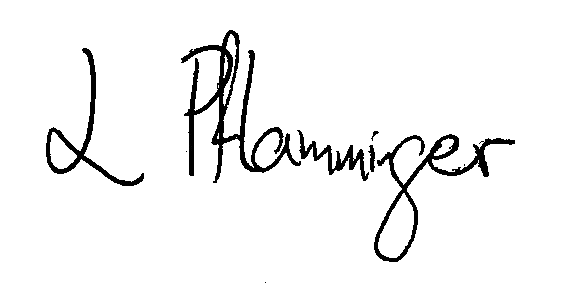
\includegraphics[width=0.35\textwidth]{unterschrift}\vspace*{-0.35cm}
		\\
		\rule[0.5ex]{12em}{0.55pt} & \rule[0.5ex]{12em}{0.55pt} \\
		(Ort, Datum) & (Eigenhändige Unterschrift)
		\\
	\end{tabular*} \\
\end{table}

\newpage


%-----------------------------------
% Seitennummerierung auf arabisch und ab 1 beginnend umstellen
%-----------------------------------
\pagenumbering{arabic}
\setcounter{page}{1}

%-----------------------------------
% Kapitel / Inhalte
%-----------------------------------
% Die Kapitel werden über folgende Datei eingebunden
% Hinzugefügt aufgrund von Issue 167
%-----------------------------------
% Kapitel / Inhalte
%-----------------------------------
% this file is imported into thesis_main.tex
% the section files are not imported directly!

\section{Einleitung}

\subsection{Problemstellung}

Das Geschäftliche Umfeld moderner Unternehmen ist wechselhaft und komplex.
Kundenanforderungen sowie Marktbedingungen verändern sich stetig und der Hohe Grad an
Vernetzung zwischen verschiedenen Anwendungen erschwert die Übersicht.
Aufgrund dieser schweren Bedingungen, benötigen große Softwareunternehmen wie
Microsoft oder Alphabet Möglichkeiten, schnell auf sich ändernde Bedingungen zu reagieren,
Kundenanforderungen rasant umzusetzen und die Zusammenarbeit und Wissensverteilung effizient
zu organisieren. In dieser Arbeit wird untersucht, ob das Konzept DevOps plausible
Chancen bietet, um diesen hohen Anforderungen gerecht zu werden.

\subsection{Zielsetzung}

Ziel dieser Arbeit ist es, die Prinzipien des DevOps Konzepts im Software Engineering
zu beschreiben, sowie seine Chancen für Unternehmen und Entwicklungsteams darzulegen.
Zudem soll DevSecOps thematisch eingeordnet werden. 

\subsection{Aufbau der Arbeit}

Die Arbeit beginnt mit einer Darstellung und Erklärung des Software Lebenszyklus und seiner
Schritte. Anschließend wird das Wasserfallmodell als Beispiel für ein konventionelles Ablaufmodell
erläutert. Agile Entwicklung wird abgegrenzt und anhand von Scrum erklärt.
Im Hauptteil wird zunächst der Begriff DevOps definiert und Ursprung und Ziel des Konzepts
erläutert. Anschließend werden die Grundsätze von DevOps anhand der sechs Säulen dargelegt.
Nachdem die Prinzipien von DevOps klar sind, werden Chancen gegeben, die DevOps modernen
Softwareunternehmen bietet. Daraufhin wird der Begriff DevSecOps im Kontext von DevOps eingeordnet.
Abschließend werden die Erkenntnisse zusammengefasst und mögliche Kritik am Konzept adressiert.
\section{Grundlagen}
\newpage
\section{Prinzipien und Chancen von DevOps}

\subsection{Definition und Ziel von DevOps}

Der Begriff DevOps setzt sich aus den Begriffen Development und 
Operations (engl. Betrieb) abgeleitet ist \cite{Alt2017}.
Development steht dabei für die Softwareentwicklung,
während Operations für den IT-Betrieb steht \cite{DevOpsAgileHeroes}.

DevOps ist eine Kombination von kulturellen und organisatorischen Denkweisen,
Prozessen und Tools, die darauf ausgerichtet sind, den Zeitraum zwischen 
der Planung und Entwicklung einer Änderung an der Software,
bis zur Bereitstellung dieser
Änderung für Kunden auf dem Produktivsystem möglichst weit zu verringern \cite{AmazonDevOps}.
Eine Änderung kann dabei ein neues Produkt, Feature oder das Beheben eines Fehlers sein.
Durch diese erhöhte Geschwindigkeit können Unternehmen die Time-to-Market,
also die Zeit, bis ein neues Feature oder Produkt den Markt erreicht,
drastisch reduzieren, was es ihnen in erster Linie erlaubt,
schnell auf Feedback der Kunden und Veränderungen auf dem Markt reagieren zu können,
um einen Wettbewerbsvorteil zu erlangen. Auch Fehler können schneller angegangen werden,
was eine kontinuierliche Verbesserung des Service zur Folge hat \cite{Halstenberg2020}.

DevOps nahm seinen Ursprung bei einer Konferenz in 2009, bei der das Team von Flickr
einen Prozess vorstellte, mit dem es in der Lage ist, neue Änderungen an der Software
bis zu zehn mal am Tag in das Produktionssystem zu übernehmen.
Inspiriert ist die Bewegung auch durch das \ac{TPS}, welches durch
T. Ohno bei Toyota entwickelt wurde \cite{Halstenberg2020}.
Es ist ein Produktionssystem in der Autoindustrie, das einzig darauf ausgerichtet ist,
den Moment zwischen dem Kundenauftrag und dem Geldeingang zu minimieren.
Konzepte aus \ac{TPS} wurden auf den IT-Wertschöpfungsprozess umgelegt,
um von den gleichen Vorteilen profitieren zu können \cite{Halstenberg2020}.

DevOps stellt keinen festgelegten Standard, wie z.B. SCRUM dar,
sondern entwickelt sich kontinuierlich weiter.
Es beruht auf bereits etablierten Konzepten wie Agilität, IT-Service Management,
KanBan und Automatisierung. Dabei erfindet es diese Konzepte nicht neu, sondern bietet
die Möglichkeit, sie zu nutzen, um eine Brücke zwischen den drei Seiten 
Entwicklung, Betrieb und Business zu schaffen \cite{Halstenberg2020}

\subsection{Die Säulen von DevOps}

Das Akronym \ac{CAMS}, oder erweitert \ac{CALMAS}, wird verwendet, um
Einige Grundsätze von DevOps zusammenzufassen.

\textbf{Culture} (Kultur):

Die Kultur im Unternehmen und im Team ist ein wichtiger Bestandteil von DevOps.
Grundlage der Kultur ist die intensive Zusammenarbeit miteinander.
Die Gewinnung und das Verteilen von Informationen wird gefördert. Das Überbringen
schlechter Nachrichten ist wichtig und wird befürwortet, um Fehler schnell beheben
zu können. Dabei werden diese nicht verurteilt oder bestraft, sondern untersucht und
korrigiert. Risiken werden geteilt und abteilungsübergreifendes Handeln wird gefördert.
Ein wichtiger Teil der Kultur ist es zudem, ständig neue Ansätze auszuprobieren,
um sich kontinuierlich weiterzuentwickeln \cite{Halstenberg2020}.

\textbf{Automation} (Automatisierung):

Die gesamte Kette des Softwareentwicklungsprozesses sollte automatisiert abgebildet werden.
Dies wird über sog. \ac{CI/CD} Pipelines realisiert und umfasst unter anderem 
automatisierte Tests, Bereitstellung und Produktivnahme der Software.
Durch Automatisierung können Liegezeiten und Fehler vermieden, sowie
Entlastung bei den Mitarbeitern geschaffen werden \cite{Alt2017}\cite{Halstenberg2020}.

\textbf{Lean}:

Lean-Methoden umfassen vor allem leichtgewichtige Entscheidungsprozesse, kontinuierliche
Messungen und die Visualisierung von Arbeit.
Auch die Limitierung von Work-in-Progress Items ist wichtig um Durchlaufzeiten zu verringern.
Sie begrenzen die Anzahl an Aufgaben, die ein Mitarbeiter oder das gesamte Team
gleichzeitig in Bearbeitung haben darf \cite{Halstenberg2020}.

\textbf{Measurement} (Messung):

Um die Produktivität des DevOps Prozesses steigern zu können, sind \acp{KPI} nötig,
um die Leistung des Teams einstufen und messbare Ziele definieren zu können.
Interessante Kennzahlen sind dabei z.B. Verfügbarkeiten, die Dauer vom Auftreten
eines Fehlers bis zur Behebung oder die Zeit von einer Änderung im Code, bis diese in
der Produktion zu sehen ist.
Zudem sind Kennzahlen, die den geschäftlichen Nutzen der IT messen wichtig \cite{Halstenberg2020}.

\textbf{Added Value} (Mehrwert):

DevOps darf nur eingesetzt werden, wenn es einen konkreten Mehrwert für das Unternehmen
bringt. Ein gutes Beispiel für solch einen Mehrwert, ist die schnellere Auslieferung
eines Features an einen Kunden oder das schnellere Beheben eines Fehlers \cite{Halstenberg2020}.
Kann kein messbarer Mehrwert festgestellt werden, wurde DevOps nicht erfolgreich implementiert.


\textbf{Sharing} (Teilen):

Eng mit dem Punkt "Culture" ist auch der Punkt "Sharing" verbunden.
Er beschreibt das Prinzip des Teilens von für die Zusammenarbeit notwendigem Wissen
mit allen Beteiligten Mitarbeitern. Dieses Wissen kann die das Produkt selbst,
aber auch Prozesse und Tools, die den DevOps Prozess erleichtern, umfassen.
Wie bereits genannt ist das Teilen von Fehlern auch ein zentraler Bestandteil und
muss ohne Schuldzuweisungen, sondern Lösungsorientiert, erfolgen \cite{Halstenberg2020}.

\subsection{Chancen von DevOps}

Die heutige Geschäftsumgebung lässt sich gut durch das Akronym \ac{VUCA} darstellen,
welches Zusammengefasst folgende Punkte beinhaltet.
Die Märkte und Kundenanforderungen sind wechselhaft und verändern sich ständig.
Dadurch entsteht eine gewisse Unsicherheit, die es erschwert, langfristige Projekte
und Strategien zu planen \cite{Halstenberg2020}.
Mit dem hohen Grad an Vernetzung zwischen verschiedenen Anwendungen und Prozessen
geht eine hohe Komplexität einher. Der Zusammenhang zwischen Ursache und Wirkung
ist oft unklar. Zudem sind meist verschiedene Handlungsalternativen als Antwort
auf bestimmte Informationen möglich, da diese durch komplexe Zusammenhänge
oft mehrdeutig interpretiert werden können \cite{Halstenberg2020}.

DevOps bietet eine Antwort auf fast alle dieser Punkte und bietet somit die Chance,
in einer VUCA-Welt geschäfts- und handlungsfähig zu bleiben.

Durch die hohe Geschwindigkeit ist DevOps in der Lage, die Time-to-Market erheblich
zu senken. In einer VUCA-Welt hat dies mehrere Vorteile.
Zum einen kann wesentlich schneller auf Veränderungen im Markt reagiert werden,
da die Durchlaufzeit von Anpassungen am Produkt oder neuen Features geringer ist.
Dies erhöht die Chance, dass Kundenanforderungen nicht bereits veraltet sind,
wenn die Änderungen fertiggestellt werden \cite{Halstenberg2020}

Durch die rasche Bereitstellung verringert sich auch die Time-to-Value, das heißt die 
Zeit, bis der Kunde einen ersten Mehrwert aus einem Produkt ziehen kann.
Dies wird durch das kontinierliche Deployment neuer Änderungen erreicht. So erhält
der Kunde zu Anfang zwar kein fertiges Produkt, kann aber bereits Vorteile aus einem
Prototypen ziehen \cite{Halstenberg2020}. Zudem verringert sich so die Zeit, bis Feedback eingeholt werden kann
was Unsicherheit und Komplexität verringert und Planungssicherheit gibt.

Die verbesserte Zusammenarbeit innerhalb cross-funktionaler Teams mit guter Kultur
kann helfen, die Komplexität und Ambiguität des Geschäftsumfelds zu verringern.
Bessere Kommunikation und unterschiedliche Skillsets ermöglichen einen besseren Überblick
über verschiedene Handlungsoptionen und erleichern die Entscheidungsfindung.

Abgesehen von VUCA bietet DevOps weitere Chancen.
Die Zuverlässigkeit und Qualität kann durch automatisiertes Testing und Bereitstellung
erhöht werden. Durch automatisierte Prozesse wird die Fehleranfälligkeit
reduziert und die allgemeine Codequalität steigt \cite{AmazonDevOps}.

Durch automatisierte Prozesse ist sichergestellt, dass auch Projekte mit großem 
Umfang zügig bereitgestellt werden können. Dies ist möglich, da Automatisierungen und die 
unterliegende virtuelle Infrastruktur sehr gut skalieren können \cite{AmazonDevOps}.

Eine weitere Chance, die DevOps bietet, ist erhöhte Sicherheit.
Diese wird vor allem im erweiterten Modell DevSecOps mit in Betracht gezogen,
welches nachfolgend eingeordnet wird.

\subsection{Einordnung von DevSecOps}

DevSecOps erweitert den DevOps Gedanken um ein weiteres Themenfeld, die Sicherheit oder
Security. In diesem Ansatz ist die Software Sicherheit ein integraler Bestandteil
des IT-Lifecycles \cite{RedHatDevSecOps}.
Traditionell ist IT-Security eine abgetrennte, der Softwareentwicklung nachgelagerte Funktion
und Aufgabe eines seperaten Teams.
Mit schnellen Entwicklungszyklen, wie sie DevOps bietet, ist das Risiko groß,
dass die Sicherheit den Entwicklungs- und Bereitstellungsprozess ausbremst, da
sie nicht schnell genug auf Veränderungen reagieren kann \cite{RedHatDevSecOps}.

DevSecOps berücksichtigt die Anwendungssicherheit von Anfang an. Dies beinhaltet die
Automatisierung von sicherheitsrelevanten Tests und Prozessen,
um den DevOps Prozess nicht zu verlangsamen und Releasezyklen schnell zu halten.
Neben zusätzlicher Automatisierung und Tools ist aber auch ein Kulturwechsel nötig.
Sicherheitsteams müssen von Beginn an fest mit in den Prozess integriert werden.
Entwickler müssen offen mit Sicherheitsexperten kommunizieren und Bedrohungen müssen
offen Kommuniziert werden, ähnlich der Fehlerkultur im regulären DevOps \cite{RedHatDevSecOps}.
\section{Zusammenfassung und Fazit}

Die Ergebnisse dieser Arbeit zeigen, dass DevOps verschiedene
Methoden, Prozesse, Tools und Denkweisen in sich vereint, um
die Geschwindigkeit des Softwareentwicklungsprozesses 
und der Bereitstellung von Software zu erhöhen.
Cross-funktionale Teams, eine collaborative Kultur,
ein hoher Automatisierungsgrad, KPIs zur Erfolgsmessung und
Arbeitsvisualisierung sowie das Teilen neuer Erkenntnisse sind
Kernbestandteile von DevOps.
Diese Prinzipien bieten viele Chancen für Unternehmen, wie
schnellere Reaktionen auf Kundenanforderungen oder Veränderungen
am Markt, Reduktion von Komplexität und Unsicherheit oder
bessere Übersicht und Entscheidungsfindung durch effizientere
Zusammenarbeit. Zum Schluss wurde DevSecOps erläutert und eingeordnet.

Zusätzlich zu den Chancen, die in dieser Arbeit dargestellt wurden
gibt es aber auch Kritik am DevOps Konzept.
So gibt es Stimmen die behaupten, dass DevOps nicht funktioniere,
da es in einer überwiegenden Anzahl an Unternehmen nicht die gewünschten
Ergebnisse bringe \cite{Halstenberg2020}.
Eine andere These ist, dass DevOps sich in vielen Bereichen nicht mit der
Regulatorik vereinbaren lässt, z.B. im Bankensektor, in dem feste Rahmenbedingungen
für die Durchführung und Dokumentation von Softwareprojekten existieren.
Es wird zudem behauptet, dass DevOps nicht in der Lage ist, Silos aufzubrechen, sondern
diese lediglich verschiebt \cite{Halstenberg2020}.

Trotz dieser Kritikpunkte wird DevOps in den größten Softwareunternehmen eingesetzt
und sorgt dafür, dass die Entwicklung mit der schnellebigen modernen Welt mithalten
kann. Jede IT-Abteilung sollte Prüfen, ob sich durch den Einsatz von DevOps Prinzipien
ein wirtschaftlicher und organisatorischer Vorteil erreichen lässt.




%-----------------------------------
% Apendix / Anhang
%-----------------------------------
%\newpage
%\section*{\AppendixName} %Überschrift "Anhang", ohne Nummerierung
%\addcontentsline{toc}{section}{\AppendixName} %Den Anhang ohne Nummer zum Inhaltsverzeichnis hinzufügen
%
%\begin{appendices}
%% Nachfolgende Änderungen erfolgten aufgrund von Issue 163
%\makeatletter
%\renewcommand\@seccntformat[1]{\csname the#1\endcsname:\quad}
%\makeatother
%\addtocontents{toc}{\protect\setcounter{tocdepth}{0}} %
%	\renewcommand{\thesection}{\AppendixName\ \arabic{section}}
%	\renewcommand\thesubsection{\AppendixName\ \arabic{section}.\arabic{subsection}}
%	\section{Anhang}
%\end{appendices}
%\addtocontents{toc}{\protect\setcounter{tocdepth}{2}}

%-----------------------------------
% Literaturverzeichnis
%-----------------------------------
\newpage

% Die folgende Zeile trägt ALLE Werke aus literatur.bib in das
% Literaturverzeichnis ein, egal ob sie zietiert wurden oder nicht.
% Der Befehl ist also nur zum Test der Skripte sinnvoll und muss bei echten
% Arbeiten entfernt werden.
%\nocite{*}

%\addcontentsline{toc}{section}{Literatur}

% Die folgenden beiden Befehle würden ab dem Literaturverzeichnis wieder eine
% römische Seitennummerierung nutzen.
% Das ist nach dem Leitfaden nicht zu tun. Dort steht nur dass 'sämtliche
% Verzeichnisse VOR dem Textteil' römisch zu nummerieren sind. (vgl. S. 3)
%\pagenumbering{Roman} %Zähler wieder römisch ausgeben
%\setcounter{page}{4}  %Zähler manuell hochsetzen

% Ausgabe des Literaturverzeichnisses

% Keine Trennung der Werke im Literaturverzeichnis nach ihrer Art
% (Online/nicht-Online)
%\begin{RaggedRight}
%\printbibliography
%\end{RaggedRight}

% Alternative Darstellung, die laut Leitfaden genutzt werden sollte.
% Dazu die Zeilen auskommentieren und folgenden code verwenden:

% Literaturverzeichnis getrennt nach Nicht-Online-Werken und Online-Werken
% (Internetquellen).
% Die Option nottype=online nimmt alles, was kein Online-Werk ist.
% Die Option heading=bibintoc sorgt dafür, dass das Literaturverzeichnis im
% Inhaltsverzeichnis steht.
% Es ist übrigens auch möglich mehrere type- bzw. nottype-Optionen anzugeben, um
% noch weitere Arten von Zusammenfassungen eines Literaturverzeichnisse zu
% erzeugen.
% Beispiel: [type=book,type=article]
\printbibliography[nottype=online,heading=bibintoc,title={\langde{Literaturverzeichnis}\langen{Bibliography}}]

% neue Seite für Internetquellen-Verzeichnis
\newpage

% Laut Leitfaden 2018, S. 14, Fussnote 44 stehen die Internetquellen NICHT im
% Inhaltsverzeichnis, sondern gehören zum Literaturverzeichnis.
% Die Option heading=bibintoc würde die Internetquelle als eigenen Eintrag im
% Inhaltsverzeicnis anzeigen.
%\printbibliography[type=online,heading=bibintoc,title={\headingNameInternetSources}]
\printbibliography[type=online,heading=subbibliography,title={\headingNameInternetSources}]

\newpage
\pagenumbering{gobble} % Keine Seitenzahlen mehr

%-----------------------------------
% Ehrenwörtliche Erklärung
%-----------------------------------
\section*{%
	\langde{Ehrenwörtliche Erklärung}
	\langen{Declaration in lieu of oath}}
\langde{Hiermit versichere ich, dass die vorliegende Arbeit von mir selbstständig und ohne unerlaubte Hilfe angefertigt worden ist, insbesondere dass ich alle Stellen, die wörtlich oder annähernd wörtlich aus Veröffentlichungen entnommen sind, durch Zitate als solche gekennzeichnet habe. Ich versichere auch, dass die von mir eingereichte schriftliche Version mit der digitalen Version übereinstimmt. Weiterhin erkläre ich, dass die Arbeit in gleicher oder ähnlicher Form noch keiner Prüfungsbehörde/Prüfungsstelle vorgelegen hat. Ich erkläre mich damit einverstanden, dass die Arbeit der Öffentlichkeit zugänglich gemacht wird. Ich erkläre mich damit einverstanden, dass die Digitalversion dieser Arbeit zwecks Plagiatsprüfung auf die Server externer Anbieter hochgeladen werden darf. Die Plagiatsprüfung stellt keine Zurverfügungstellung für die Öffentlichkeit dar.}
\langen{I hereby declare that I produced the submitted paper with no assistance from any other party and without the use of any unauthorized aids and, in particular, that I have marked as quotations all passages which are reproduced verbatim or near-verbatim from publications. Also, I declare that the submitted print version of this thesis is identical with its digital version. Further, I declare that this thesis has never been submitted before to any examination board in either its present form or in any other similar version. I herewith agree that this thesis may be published. I herewith consent that this thesis may be uploaded to the server of external contractors for the purpose of submitting it to the contractors’ plagiarism detection systems. Uploading this thesis for the purpose of submitting it to plagiarism detection systems is not a form of publication.}


\par\medskip
\par\medskip

\vspace{5cm}

\begin{table}[H]
	\centering
	\begin{tabular*}{\textwidth}{c @{\extracolsep{\fill}} ccccc}
		\myOrt, \the\day.\the\month.\the\year
		&
		% Hinterlege deine eingescannte Unterschrift im Verzeichnis /abbildungen und nenne sie unterschrift.png
		% Bilder mit transparentem Hintergrund können teils zu Problemen führen
		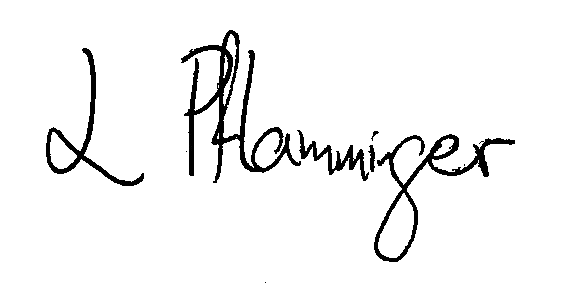
\includegraphics[width=0.35\textwidth]{unterschrift}\vspace*{-0.35cm}
		\\
		\rule[0.5ex]{12em}{0.55pt} & \rule[0.5ex]{12em}{0.55pt} \\
		\langde{(Ort, Datum)}\langen{(Location, Date)} & \langde{(Eigenhändige Unterschrift)}\langen{(handwritten signature)}
		\\
	\end{tabular*} \\
\end{table}

\end{document}
